\chapter{Methods}\label{ch3}

In this chapter, our main contributions are elaborated. We explain in detail our proposed method of the fitting pipeline, including its key components that we have put together to build the module based coherent and reliable system. The overview diagram of the system we have implemented can be seen in Figure \ref{flow}. The system makes sure that the data from the camera is seamlessly delivered to the fitting pipeline in the correct format and being utilized efficiently. Further, in this chapter, we describe each of the key components of the system that could be split into three distinct modules:
\begin{enumerate}[$\bullet$]
    \item Module 1: takes care of the camera configuration, data capturing and preprocessing procedure (Figure \ref{flow} \textbf{Server} block). Among others, the data capturing procedure includes the acquisition of 3D landmarks, which introduces an additional technical challenge since they are not directly obtainable from the camera. 
    \item Module 2: receives the data from the server, processes it, and performs the shape fitting (Figure \ref{flow} \textbf{Client \& Shape Fitting} blocks\footnote{In practice, these two modules are merged into one, we split them here to make procedures clear.}). Besides the more important shape fitting procedure, this module also takes care of minor but nevertheless important aspects of the module, such as data conversion and cleaning.
    \item Module 3: receives the best shape fit produced by the shape fitting module, alongside other necessary data, and performs the color fitting (Figure \ref{flow} \textbf{Color Fitting} block). The color fitting performed in this module is very much like the standard fitting approach, except small modifications as we discuss them in the following chapters.
\end{enumerate}    

In this way, it is very easy to control and use those modules for specific applications, like only producing the data and using it for other purposes, or only obtaining the shape fit where the color fit is not required. \bigskip

We first explain in detail the camera calibration and configuration procedure. Then we introduce the software development kit that allows us to communicate with the camera and perform the data acquisition procedure. Further, the client-server API is introduced. Based on this API data is seamlessly being delivered to the module that utilizes it. We also describe the data capturing procedure alongside the client-server interaction. Finally, and most importantly both of our fitting modules are elaborated, including the description of the proposals and evaluators used.


\begin{figure}
  \centering
  \includegraphics[width=\textwidth]{Figures/FittingFlowNew.pdf}
  \caption{An overview of our system with its key modules and procedures.}
  \label{flow}
\end{figure}

\section{Camera}
Before we start working on our project is it essential to configure and calibrate the camera in order to maximize its performance. As we have mentioned previously, our camera of choice is the Intel® RealSense™ D415 depth camera. Thanks to its rolling shutter and narrow field of view, the camera is focused on accuracy and is especially well suited for near and still object scanning applications. 

\subsection{Camera Calibration}
To calibrate the camera we use Intel's Dynamic Calibrator tool. The camera can be calibrated by either displaying a calibration texture pattern on a mobile device screen or printing it on a white paper and following the Calibrator tool instructions (Figure \ref{f3.1}). Dynamic calibration tool optimizes the cameras' extrinsic parameters with regard to the main axis, consisting of rotation and translation parameters\cite{cal}. 

\begin{figure}
  \begin{minipage}{.49\textwidth}
    \includegraphics[width=0.99\textwidth]{Figures/Pictures/cal1.png}
  \end{minipage}
  \begin{minipage}{.49\textwidth}
    \includegraphics[width=0.99\textwidth]{Figures/Pictures/cal2.png}
  \end{minipage}
  \caption{Left: Rectification phase, Right: Scale phase. Source: Intel}
  \label{f3.1}
\end{figure} 

To evaluate the performance of our camera after the calibration procedure we use Depth Quality tool\footnote{\text{Depth Quality Tool} — \url{https://github.com/IntelRealSense/librealsense/tree/master/tools/depth-quality}} (Figure \ref{f3.2}). 

\begin{figure}
  \begin{minipage}{.49\textwidth}
    \centering
    \includegraphics[width=0.99\textwidth]{Figures/Pictures/dc.png}
  \end{minipage}
  \begin{minipage}{.49\textwidth}
    \centering
    \includegraphics[width=0.99\textwidth]{Figures/Pictures/ic.png}
  \end{minipage}
  \caption{Depth quality tool using Intel's recommended textured wall test method to assess performance, displaying depth (left) and infrared (right) stream view, alongside with an ROI area marked with a yellow rectangle.}
  \label{f3.2}
\end{figure}

By running a series of recommended tests we obtain a set of important quality measurements presented in Table \ref{t3.1}. \textbf{Fill rate} measures the percentage of pixels with valid depth value within the Region-Of-Interest (ROI). \textbf{Z-accuracy} indicates the depth accuracy given the Ground Truth (GT) as a percentage of the range, where positive value means that the depth plane fit is behind the ground truth (overshot), and a negative value indicates that the depth plane fit is in front of ground truth (undershot). \textbf{Plane Fit RMSE} calculates the Root-Mean-Squared (RMS) error of Z-error (Spatial noise). \textbf{Sub-pixel RMSE} provides sub-pixel RMS error.\footnote{This information is taken from the depth quality tool itself, refer to footnote link above for more details.} 


\begin{table}[h]
  \centering
  \begin{tabular}{c|c|c|c}
    Measurement  & Result & ROI & Resolution\\
    \hline
    Fill Rate   & 100\%  &40\% & 1280x720 \\ \hline
    Z-Accuracy   & 0.24\% &40\% & 1280x720 \\ \hline
    Plane Fit RMSE   & 0.24\% & 40\% & 1280x720 \\ \hline
    Sub-pixel RMSE   & 0.13\% & 40\% & 1280x720 \\ 
    \hline
  \end{tabular}
  \caption{Calibration test results.}
  \label{t3.1}
\end{table}

\subsection{Camera Configuration Parameters}
After the camera calibration, we proceed with configuring the camera parameters including resolution, stream profiles (Color and Depth stream separately), measurement distance, filters and a long set of other depth configuration parameters. If not stated otherwise we do not modify any sensitive parameter and use Intel's recommended settings as of \cite{bestcal}. Although Intel recommends to use 1280x720 image resolution for an optimal image quality and depth accuracy, we have decided to use 640x480 resolution to right away reduce the number of calculations needed to do any sort pixel-wise or point-wise operations and yet maintain a decent image quality. 1280x720 resolution yields ~900k pixels/points as opposed to ~300k in the case of 640x480. When it comes to camera stream formats we use traditional \textit{z16} format for the depth stream and \textit{rgb8} format for the color stream. We enable auto exposure setting which allows the camera to dynamically adjust exposure for the various light and illumination environments. Since our application only requires a still relatively close-up distance head shots we set the minimum depth distance to 0.2 meter and maximum distance to 1 meter as well as the ROI parameter to 40\%. This is because we are not interested in the entire scene captured by the camera but rather the face area.  As of filters, we did not make use of them because we opted to work with raw data without various filters influencing its quality.  The final note we would like to make regarding the camera configuration is that we align color and depth stream frames. The reason is straightforward, we would like to have the data that have the same view-point — color and depth frames should be in correspondence. If we do not align them, they will be viewed from slightly different angles, this is due to spatial differences between physical camera sensors. This process will become more obvious in Section \ref{s3.3.2} were we describe the process of capturing 3D landmarks. 

\subsection{SDK}\label{s3.1.3}
To take advantage of the camera hardware and to fit the capture procedure to our needs we have to use Intel's \textit{librealsense}\footnote{Intel® RealSense™ SDK — \url{https://github.com/IntelRealSense/librealsense}} SDK. The reason why it is necessary to communicate with the camera through the API instead of using Intel's RealSense Viewer (Figure \ref{f3r}) is that firstly, it does not provide all the required data out-of-the-box and secondly, the data cannot be captured all at once. As we are designing our system to work in a variety of application scenarios including a web environment, it is crucial to automate all parts and run the system with minimal to no human interaction. \bigskip

\begin{figure}[ht!]
  \centering
  \includegraphics[width=0.98\textwidth]{Figures/Pictures/rsviewer.png}
  \caption{Intel RealSense Viewer — 3D Depth View with camera configuration parameters on the left side. Blue color indicates near points, red — far.}
  \label{f3r}
\end{figure}
While being written in C++ the SDK provides wrappers for the majority of the popular programming languages\footnote{Not all wrappers support full features offered by the native SDK}. Unfortunately, Java Virtual Machine (JVM) based languages (one of which, namely Scala we are going to use in the main part of the project) are not officially supported. Therefore, we had to choose an alternative lightweight and fast language, flexible enough to seamlessly run on any machine and operating system. We have decided to use Python because of its powerful companion frameworks, ease of use and also because of \textit{pyrealsense2} — librealsense's Python wrapper that is stable and relatively fully featured comparing to others. We hereby note that upon investigating the camera SDK we have discovered\footnote{GitHub Issue — \url{https://github.com/IntelRealSense/librealsense/issues/3716}} that it does not have a dedicated computer vision middleware module it used to have in the previous generation \cite{betschard2016} used. The module used to offer relevant features for our application such as face scanning and landmark detection. Not having a direct, native access to these features introduces additional technical challenge. Since the performance of or application crucially depends on a set of facial landmarks we had to find a way to detect them. We present our solution to this problem in Section \ref{s3.3} where we describe a complete data acquisition procedure. The one last important notice we would like to make regarding the choice we have made in this section is that obviously, we cannot simply communicate between Python and Scala code base. To deal with cross-language modules we rely on interface definition language framework — Apache Thrift\footnote{Apache Thrift™ — \url{https://thrift.apache.org}}.  

\section{Cross-Language API}
\begin{figure}
  \centering
  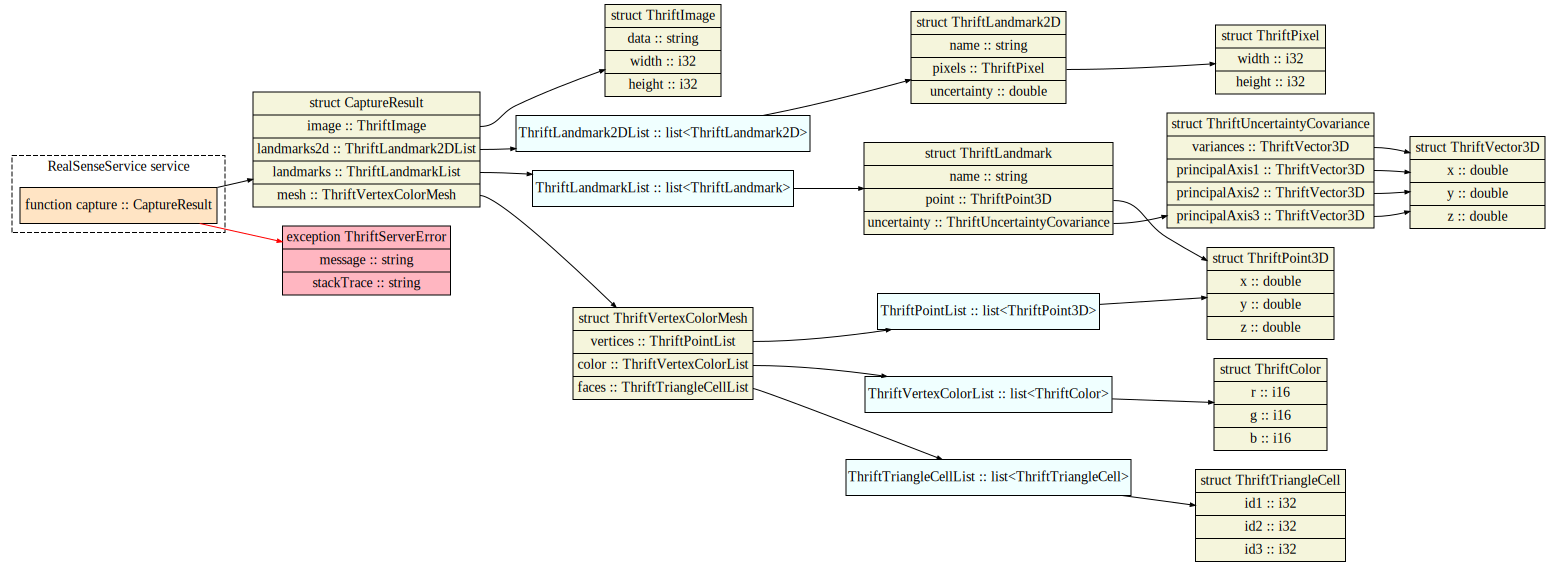
\includegraphics[width=\textwidth]{Figures/thrift/Rs-ex.pdf}
  \caption{Diagram of our API. *For better resolution please refer to Appendix \ref{fA.1}}
  \label{f3.3}
\end{figure}

Thrift is an interface definition language designed to solve the problem of sharing the code base of cross-language modules. Specifying the signature of all the important types, methods and exceptions in the thrift interface — the framework generates an identical API for any major programming languages. By doing so, Thrift takes care of all the language specific details such as syntax, type variations, exceptions, etc. and makes sure that the code generated for the different languages are usability-wise identical from an API consumer's perspective. The diagram of our thrift interface can be seen in Figure \ref{f3.3}. We define a set of relevant data structures such as \textit{Pixel, Point, Vector, Image, Landmark, Triangle} and \textit{Color} with respective lists that utilize some of those values \textit{PointList, LandmarkList, ColorList}, and \textit{TriangleList}. We also define a mesh structure with signature \textit{TriangleMesh(PointList, ColorList, TriangleList)}, as well as, the main data holder object \textit{CaptureResult(Image, Landmark2D, Landmark3D, TriangleMesh)}. \textit{CaptureResult} is the object that is being passed from the server-side to the client-side. Every mentioned data type has its respective converter method implemented in both Python and Scala code base. We did not make use of 2D landmarks in this project, so we do not pay attention to it any further, however, if needed — its functionality is fully implemented in both Python and Scala code. 


\section{Capture Procedure (Server)}\label{s3.3}

\begin{figure}
  \centering
  \includegraphics[width=0.5\textwidth]{Figures/Server.pdf}
  \caption{The server diagram.}
  \label{server}
\end{figure}

Upon receiving a request our server (Figure \ref{server}) launches a pre-configured camera stream into the OpenCV\footnote{Open Source Computer Vision Library — \url{https://opencv.org/}} window (Figure \ref{f3.5}) that is split into two sub-windows, one displaying an RGB color stream and the other depth stream. Red color indicates pixels that are closer to the camera and blue that are farther. Note that the server does not execute capturing once it receives the request, instead it runs the camera stream and waits for additional user input (for example pressing the “D” key on the keyboard). This is because otherwise, the user will not be able to adjust their position. Obviously, it is possible to add timeout before capturing but having a visual tool is still preferred.  Once the server receives a call to run the capturing script, it captures the required raw data and starts processing it. For the successful pipeline run, as we have mentioned previously, our modified fitting pipeline requires the following data: \textbf{RGB Color Image}, \textbf{A Set of 3D Landmarks} and \textbf{Point Cloud Mesh}.

\begin{figure}
  \centering
  \includegraphics[width=\textwidth]{Figures/Pictures/no-glasses.png}
  \caption{The OpenCV window displaying an RGB color image (left) and the depth image (right) visualized using JET color map. }
  \label{f3.5}
\end{figure}

\subsection{RGB Color Image}
Capturing a color image is not complicated, and we do not do any post-processing to it. After converting it to the Thrift image type using the corresponding converter method we directly pass it to the \textit{CaptureResult} object described above.

\subsection{3D Landmarks}\label{s3.3.2}
Obtaining 3D landmarks is one of the important data requirements for this project. The problem arose due to the lack of 3D landmark availability in the SDK. The solution to this problem we have implemented is to detect 2D (pixel) landmarks on the color image using Dlib\footnote{Dlib C++ library — \url{http://Dlib.net}} landmark detection library (Figure \ref{f3.6}). These landmarks are then de-projected into 3D landmark points using the camera SDKs de-projection capabilities we discussed previously. The de-projection is based on camera settings for the specific session (shot).

\begin{figure}[h]
  \centering
  \includegraphics[width=\textwidth]{Figures/Pictures/lmoverlay.png}
  \caption{Facial landmark detection using OpenCV and Dlib libraries visualized over D415's color stream.}
  \label{f3.6}
\end{figure}

Dlib landmarks usually have corresponding landmark ID assigned to it, based on those IDs we match each 2D landmark to the fitting pipeline landmarks by the name. This way, after performing de-projection we create the landmark structure that corresponds to the structure defined in the fitting pipeline \textit{\{"landmarkID": [$LM_x, LM_y, LM_z$]\}}. Sometimes detected pixel landmarks do not have corresponding 3D point due to missing depth information, in situations like this 3D landmark points will be filled with 0.0 values. We will deal with these landmarks on the client-side where we determine which landmarks to use. During landmark de-projection, it is essential to have color and depth frames in correspondence (aligned). Otherwise, when examining point cloud, landmarks will not appear in locations where they supposed to, because point cloud mesh will be captured based on depth stream and landmarks will be obtained via de-projecting color stream pixels to 3D points. We have already emphasized the importance of 3D landmarks in our application, therefore, we place a hard constraint over this block of information. If Dlib for some reason fails to detect the face in the image, the capturing process throws an exception. Furthermore, when there is more than one face detected in the image, we also break the process, because the pipeline would not be able to figure out which face we are trying to reconstruct. 


\subsection{Point Cloud}\label{s3.3.3}
The camera SDK does provide raw point cloud access out-of-the-box, however, the operations that are defined on top of point cloud objects are limited to accessing the point information, saving them as a structured mesh file, obtaining texture coordinates and getting the size of a point cloud. Saving the point cloud as a mesh file is the feature we need, however, we have to modify it, because we do not save the mesh file anywhere, instead serialize and sent it through the network. We have implemented an overridden version of the mesh formation in order to satisfy this requirement. 

\begin{figure}
  \centering
  \begin{minipage}{.5\textwidth}
    \centering
    \includegraphics[width=\textwidth]{Figures/Pictures/pts1.png}
  \end{minipage}%
  \begin{minipage}{.5\textwidth}
    \centering
    \includegraphics[width=\textwidth]{Figures/Pictures/pts.png}
  \end{minipage}
  \caption{Obtained point cloud clipped at face region.}
\end{figure}

The method takes point cloud provided from the SDK and creates triangles between neighboring points. Triangle formation itself is based on the same algorithm Intel uses to save the mesh as a file. That is, we only modify the usability of the method but the algorithm is unchanged. 

\begin{figure}
  \centering
  \begin{minipage}{.32\textwidth}
    \centering
    \includegraphics[width=0.99\textwidth]{Figures/Pictures/full_pc.png}
    \caption*{(a)}
  \end{minipage}
  \begin{minipage}{.32\textwidth}
    \centering
    \includegraphics[width=0.99\textwidth]{Figures/Pictures/full_with_overlay.png}
    \caption*{(b)}
  \end{minipage}
  \begin{minipage}{.32\textwidth}
    \centering
    \includegraphics[width=0.99\textwidth]{Figures/Pictures/clip.png}
    \caption*{(c)}
  \end{minipage}
  \caption{(a) Full scene point cloud mesh. (b) The same scene as (a) but with region of interest highlighted in green. (c) Clipped face region (target mesh)}
  \label{f3.8}
\end{figure}

The point cloud obtained from the SDK contains points which are describing the entire scene most of which we are not interested in, and more importantly having unnecessary points introduces additional computational overhead during the fitting. Therefore, we consider clipping the point cloud in the face region and discard the rest of the points. This process happens on the client-side which we yet to describe. The basic flow of mesh clipping operation is shown in Figure \ref{f3.8}. We will describe this process further in Section \ref{s3.4.1}. 


\section{Fitting Pipeline (Client)}\label{s3.4}

\begin{figure}
  \centering
  \includegraphics[width=0.5\textwidth]{Figures/Client.pdf}
  \caption{The client diagram.}
  \label{client}
\end{figure}

As described previously, the fitting pipeline is split into two parts. The first part (Figure \ref{client}) is responsible for receiving the data from the server, converting it to respective Scalismo\footnote{Scalismo — Scalable Image Analysis and Shape Modelling \url{https://scalismo.org/}} objects (\textit{PixelImage, Landmark3D, TriangleMesh}), performing the necessary data cleansing procedure, and finally starting the shape fitting process. The shape fitting utilizes additional point cloud information by fitting the 3DMM onto the point cloud to obtain better pose and shape model parameters. We describe this process in Section \ref{s3.4.2}.  The second part of our proposed fitting pipeline is the color fitting stage. It is a continuation of the shape fitting in the sense that it takes the result of the shape fitting as an input, and runs the slightly modified standard color fitting. This process is described in Section \ref{s3.4.3}.

\subsection{Data Processing}\label{s3.4.1}
Before shape fitting starts it is necessary to process and clean the data received from the server. The more important data cleansing happening with \textit{Landmark3D} and \textit{TriangleMesh} structures. Before we do that, we augment the current model with additional chin landmarks that we are getting from the Dlib, and remove some which we do not have in Dlib. To make this process better understandable we visualize landmark differences in Figure \ref{f3.9}. Where the figure on the left shows the original landmarks that are available in the model, and the figure on the right shows our version of it. It should be noted that the pose variation in the image tends to affect obtained chin landmarks significantly, and the pixel-to-point de-projection we perform further increases the uncertainty of those landmarks. Therefore, to deal with this problem we assign higher uncertainty to chin landmarks that are being received from the server. 

\begin{figure}
  \centering
  \begin{minipage}{.49\textwidth}
    \centering
    \includegraphics[width=0.98\textwidth]{Figures/Pictures/origGreen.png}
    \caption*{Original model landmarks}
  \end{minipage}
  \begin{minipage}{.49\textwidth}
    \centering
    \includegraphics[width=0.98\textwidth]{Figures/Pictures/pipelineGreen.png}
    \caption*{Landmarks we use}
  \end{minipage}
  \caption{Visualization of the differences between the original model landmarks and the landmarks we use.}
  \label{f3.9}
\end{figure}

Once we have our model ready we discard landmarks that contain 0.0 values, which were produced by de-projection due to unavailable depth information. We also discard landmark points that are being de-projected wrongly due to the occlusion or frame misalignment. This is done by evaluating each landmarks' $z$ coordinate which indicates its distance from the camera and discarding landmarks that are farther than predetermined capture distance. Additionally, we remove model landmarks that are not part of our target landmarks.  Based on cleaned up target landmarks we perform mesh clipping procedure. 

\begin{figure}
  \centering  
  \begin{minipage}{.32\textwidth}
    \centering
    \includegraphics[width=0.99\textwidth]{Figures/Pictures/mesh_r.png}
  \end{minipage}
  \begin{minipage}{.32\textwidth}
    \centering
    \includegraphics[width=0.99\textwidth]{Figures/Pictures/mesh_f.png}
  \end{minipage}
  \begin{minipage}{.32\textwidth}
    \centering
    \includegraphics[width=0.99\textwidth]{Figures/Pictures/mesh_l.png}
  \end{minipage}
  \caption{Clipped sample target mesh from different angles.}
  \label{f3.10}
\end{figure}

The basic idea is to create a box region covering the face by determining the outer most landmark positions for each dimension and ignoring all the points that lie outside this region. The result of this procedure can be seen in Figure \ref{f3.10}. The only issue with this approach is that determining outer most landmarks and slicing based on their value will slice up some part of the face if the pose is too extreme. This is because slicing operation is happening parallel to basis axes. Hence, we recommend to work with no more than $\ang{30}$ degree yaw rotations and for optimal performance frontal shots where occlusion and frame misalignment are not affecting to the landmarks. The final result of the mesh slicing and landmark filtering is shown in Figure \ref{f3.11}. 

\begin{figure}
  \centering
  \includegraphics[width=0.85\textwidth]{Figures/Pictures/targetMeshWithLandmarks_t.png}
  \caption{Sample target mesh with filtered landmarks.}
  \label{f3.11}
\end{figure}

Note that there are fewer chin landmarks available on the target mesh due to the landmark filtering process described previously. This can be explained by taking into account what we have described in Section \ref{s3.3.2}. The pixel-to-point de-projection is successful, if and only if, the camera detects the respective depth information for the specific pixel we are trying to de-project. Since chin pixels commonly suffer from occlusion, camera often is not able to detect the depth information. Hence, we have some 3D landmarks that are missing from the target mesh.   

\subsection{Shape Fitting}\label{s3.4.2}

\begin{figure}[h!]
  \centering
  \includegraphics[width=0.8\textwidth]{Figures/ShapeFitting.pdf}
  \caption{The shape fitting diagram.}
  \label{shapeF}
\end{figure}
\FloatBarrier

Before we start the shape fitting process (Figure \ref{shapeF}) itself, we first align the model and the target mesh rigidly based on landmark correspondences using rigid 3D landmark registration method. The method, which is already implemented in Scalismo, performs generalized Procrustes analysis\cite{Lorusso:1995:CFA:236190.236213} to obtain the translation and rotation parameters, which we then use to give the model a good starting position parameters. This step is required because the model is centered at the origin of the 3D coordinate system, whereas the target mesh location is determined by how far the face was from the camera when the shot was made\footnote{The camera center is located at (0, 0, 0)}. A visual example of this scenario can be seen in Figure \ref{f3.12}. 

\begin{figure}
  \centering
  \includegraphics[width=0.95\textwidth]{Figures/Pictures/modelTargetDist_t.png}
  \caption{Initial location of the model (right) and the target (left).}
  \label{f3.12}
\end{figure}

The process alternatively can be performed during the fitting process itself, but we opted to obtain necessary parameters using the rigid alignment because it is usually very fast and leads the model to a correct initial position. \bigskip

Shape fitting boils down to optimizing the set of parameters $\theta = \{\theta_S, \theta_R, \theta_T\}$ referring to the model's \textit{shape}, \textit{rotation}, and \textit{translation} parameters respectively. The shape parameter $\theta_S$ is a vector of model coefficients $\theta_S = (\alpha_0,\dots,\alpha_{199})$. The rotation parameter $\theta_R$ consists of Euler rotation angles $\theta_R = (r_\phi, r_\psi, r_\omega)$ and the translation parameter $\theta_T$ is a vector holding 3D translation information $\theta_T = (t_x, t_y, t_z)$. As we have elucidated previously, the initial rotation and translation parameters are set to be an output of rigid landmark registration procedure, which leads to the state shown in Figure \ref{f3.13}.

\begin{figure}
  \centering  
  \begin{minipage}{.32\textwidth}
    \centering
    \includegraphics[width=0.98\textwidth]{Figures/Pictures/initLAlt_t.png}
  \end{minipage}
  \begin{minipage}{.32\textwidth}
    \centering
    \includegraphics[width=0.99\textwidth]{Figures/Pictures/initFAlt_t.png}
  \end{minipage}
  \begin{minipage}{.32\textwidth}
    \centering
    \includegraphics[width=0.98\textwidth]{Figures/Pictures/initRAlt_t.png}
  \end{minipage}
  \caption{The model instance and the target mesh alignment after applying the initial $\theta$.}
  \label{f3.13}
\end{figure}

\section*{Proposal Architecture}
The proposal distribution that will be used in the Metropolis-Hastings algorithm for the shape fitting is constructed similarly to the mixture proposal distribution described previously according to Equation \ref{eq2.3}. We create a mixture of three separate proposal distributions each responsible for sampling shape, translation and rotation parameters. Separating proposals from each other not only gives us better control over the individual proposals, but it also simplifies the analysis of the process as a whole. For example, this allows us to specify the step size (standard deviation) of each proposal separately. The rotation and translation proposals both are simple Random Walk proposals with isotropic Gaussian perturbation distribution. For the shape proposal though, instead of using just Random Walk proposal we use a combination of Random Walk and Iterative Closest Point (ICP) proposals. Due to fundamental characteristics of the Random Walk proposals, that is, proposing samples without having any specific target direction, they tend to require more iterations, and therefore more time for convergence. Hence, by plugging in the ICP proposal that always moves towards the target, we reduce the number of iterations and accordingly the execution time by an order of magnitude. The final mixture proposal distribution then is as follows:

\begin{equation}
  Q(\theta' | \theta) = \frac{2}{10}Q_R(\theta' | \theta) + \frac{2}{10}Q_T(\theta' | \theta) + \frac{3}{10}Q_{S(RW)}(\theta' | \theta) + \frac{3}{10} Q_{S(ICP)}(\theta' | \theta).
\end{equation}

Where $Q_R$ is the rotation proposal, $Q_T$ translation proposal, $Q_{S(RW)}$ random walk based shape proposal and $Q_{S(ICP)}$ ICP based shape proposal. The coefficients of the proposals are $c_i$ from Equation \ref{eq2.3} indicating the probability of drawing samples from the specific proposals. 

\section*{Evaluators}
The main purpose of the evaluators is to evaluate the proposed sample $\theta$ and assess whether it should be accepted or rejected based on its posterior value $P(\theta | D) \propto P(\theta) P(D | \theta)$ as described in Section \ref{s2.2.1}. We introduce two distinct likelihood evaluators under the assumption that they are conditionally independent. Based on this assumption we combine conditionally independent likelihoods using product likelihood alongside with prior evaluator. The first evaluator we model is for the landmark correspondences. Its purpose is to measure how plausible observed $n$ landmark locations are under the influence of normal isotropic Gaussian noise assumption at every point with $\sigma = 3mm$ standard deviation:
\begin{equation}
    P(D|\theta) = \mathcal L(\theta; \ell_1, \dots, \ell_n) = \prod_{i}\mathcal N(\ell_i|\ell'_i(\theta), \sigma^2_{LM3D}).
    \label{eq3.1}
\end{equation}  
Where $\ell_i$ are observed target landmarks and $\ell'_i(\theta)$ are i-th landmarks corresponding landmark on the model instance rendered based on $\theta$ parameters. \bigskip

The second evaluator we introduce is an evaluator for uniformly sampled $n \leq model_{pts}$ points on the model instance under $\theta$, which evaluates the distance between sampled points and the closest point on the target mesh surface. The Gaussian noise assumption is known to encounter problems when dealing with outliers. We observe quite a few outliers on our target mesh, therefore, we choose to use known to be more robust Cauchy\footnote{\url{https://en.wikipedia.org/wiki/Cauchy_distribution}} distribution\cite{Schoenborn2014} noise model with scale $\gamma = 0.5$:    

\begin{equation}
  \mathcal L(\theta; p'_1(\theta), \dots, p'_n(\theta)) = \prod_i Cauchy(p'_i(\theta) |p_i, \gamma_p)
  \label{eq3.3}
\end{equation}
where $p'_i(\theta)$ are uniformly sampled points onto the model instance under $\theta$ parameters and $p_i$ are its corresponding closest points on the target surface.\bigskip

When it comes to a prior evaluator, we use zero-mean normal distribution for $\theta_T$ and $\theta_R$. As for $\theta_S$ prior, we treat the model itself as a prior observation. \cite{scalismoTut}

\subsection*{Model Decimation}
Before we put everything together and construct a Markov Chain through Metropolis-Hastings algorithm and do the inference, we have to make a small but important computationally beneficial adjustments. The model we are working on contains ~28k points and ~56k triangles. Every time we apply a parameter set $\theta$ to the model to obtain a model instance it has to calculate the new position for ~28k points. This is a computationally rather heavy task, especially when considering the fact that we do not need to execute transformation over the full set of model points. The way to overcome this problem is to introduce the standard model decimation technique, which reduces the number of points without model losing its expressive shape characteristics. We will not go into details how the decimation process works, but rather report important differences between the full model and the decimated model. In Table \ref{t3.2}  various decimation rates and the corresponding number of points and triangles are shown. Figure \ref{f3.14} shows how much the visual appearance changes after decimation. 

\begin{table}[h]
  \centering
  \begin{tabular}{c|c|c}
    Decimation Rate  & Number of Points & Number of Triangles\\
    \hline
    0   & 28588  & 56572\\
    \hline
    0.1   & 25731 & 50913 \\
    \hline
    0.3   & 20017 & 39600 \\
    \hline
    0.6   & 11467 & 22628 \\
    \hline
    0.9   & 2919 & 5657 \\
    \hline
  \end{tabular}
  \caption{The number of points and triangles after decimation.}
  \label{t3.2}
\end{table}

\begin{figure}[h]
  \centering  
  \begin{minipage}{.325\textwidth}
    \centering
    \includegraphics[width=0.99\textwidth]{Figures/Pictures/d01a_t.png}
  \end{minipage}
  \begin{minipage}{.325\textwidth}
    \centering
    \includegraphics[width=0.99\textwidth]{Figures/Pictures/d06a_t.png}
  \end{minipage}
  \begin{minipage}{.325\textwidth}
    \centering
    \includegraphics[width=0.99\textwidth]{Figures/Pictures/d09a_t.png}
  \end{minipage}
  \begin{minipage}{.325\textwidth}
    \centering
    \includegraphics[width=0.99\textwidth]{Figures/Pictures/d01_t.png}
    \caption*{0.1}
  \end{minipage}
  \begin{minipage}{.325\textwidth}
    \centering
    \includegraphics[width=0.99\textwidth]{Figures/Pictures/d06_t.png}
    \caption*{0.6}
  \end{minipage}
  \begin{minipage}{.325\textwidth}
    \centering
    \includegraphics[width=0.99\textwidth]{Figures/Pictures/d09_t.png}
    \caption*{0.9}
  \end{minipage}
  \caption{Various rates of model decimation and how they influence the appearance of the model.}
  \label{f3.14}
\end{figure}

We use the decimated model with 0.9 rate for both ICP shape proposal described previously and for the closest point evaluator (Equation \ref{eq3.3}). 

\subsection*{Metropolis-Hastings}
To recall, the Metropolis-Hastings algorithm is a method of the family of Markov Chain Monte Carlo algorithms, which is based on the acceptance-rejection sampling technique. As described in Section \ref{s2.2.1} it constructs a Markov Chain by accepting or rejecting samples drawn from a proposal distribution\cite{Schoenborn2017}.  We now have defined both a proposal distribution $Q$ (Equation \ref{eq3.1}) and a target distribution $P$ which is a product of three previously mentioned evaluators(\textit{Landmarks Evaluator}, \textit{Closet Point Evaluator}, and \textit{Prior Evaluator}). Having these two distributions is all that is needed for the Metropolis-Hastings algorithm to start the propose-and-verify cycle. Therefore, we simply pass our proposal and evaluator distributions to it. In Table \ref{t3.3} proposal acceptance ratios are shown after a test shape fitting run with 1000 iterations. As expected, our ICP proposal has higher acceptance ratios than any other proposal.  

\begin{table}[h]
  \centering
  \begin{tabular}{c|c|c}
    Proposal  & Std. Deviation & Acceptance Ratio \\
    \hline
    \textit{ShapeProposalICP}   & 0.1 & 0.6292  \\
    \hline
    \textit{ShapeProposalRW}   & 0.1 & 0.1909 \\
    \hline
    \textit{RotationProposal}   & 0.01 & 0.1428 \\
    \hline
    \textit{TranslationProposal}   & 1.0 & 0.0754 \\
    \hline
  \end{tabular}
  \caption{Proposal acceptance ratios after 1000 sampling iterations.}
  \label{t3.3}
\end{table}

The runtime of this specific run was \textit{84s} on a standard laptop computer.\footnote{Intel® Core™ - i7-8550U, 32GB RAM, Intel® UHD Graphics 620} On a better performing machine, the execution time easily falls under \textit{60s}. Decreasing the number of iterations from 1000 to 500 further reduces the time on earlier mentioned machine from \textit{84s} to \textit{56s} without sacrificing fit quality too much.\footnote{Mentioned run times are only shape fitting times without client-server protocol} We will report detailed results in the next chapter but to make the above mentioned test more clear, we provide quantitative and qualitative assessments for that specific run. 

\begin{figure}
  \centering    
  \begin{minipage}{.325\textwidth}
    \centering
    \includegraphics[width=0.99\textwidth]{Figures/Pictures/sfX.png}
    \caption*{X Slice}
  \end{minipage}
  \begin{minipage}{.325\textwidth}
    \centering
    \includegraphics[width=0.99\textwidth]{Figures/Pictures/sfY.png}
    \caption*{Y Slice}
  \end{minipage}
  \begin{minipage}{.325\textwidth}
    \centering
    \includegraphics[width=0.99\textwidth]{Figures/Pictures/sfZ.png}
    \caption*{Z Slice}
  \end{minipage}
  \caption{The white line is our target mesh, colored line is the best fit converted into the scalar mesh field with scalar distance range \textit{0.0 mm} (blue) to \textit{3.0 mm+} (red).}
  \label{f3.15}
\end{figure}

\begin{figure}
  \centering    
  \begin{minipage}{.325\textwidth}
    \centering
    \includegraphics[width=0.99\textwidth]{Figures/Pictures/gtX.png}
    \caption*{X Slice}
  \end{minipage}
  \begin{minipage}{.325\textwidth}
    \centering
    \includegraphics[width=0.99\textwidth]{Figures/Pictures/gtY.png}
    \caption*{Y Slice}
  \end{minipage}
  \begin{minipage}{.325\textwidth}
    \centering
    \includegraphics[width=0.99\textwidth]{Figures/Pictures/gtZ.png}
    \caption*{Z Slice}
  \end{minipage}
  \caption{The white line is the ground truth, colored line is the best fit converted into the scalar mesh field with scalar distance range \textit{0.0 mm}(blue) to \textit{3.0 mm+}(red).}
  \label{f3.16}
\end{figure}
The average mesh distance calculated point-wise between the best model fit and the target mesh shown in Figure \ref{f3.15} was \textbf{\textit{1.26 mm}}. The average mesh distance calculated between the same best model fit and the ground truth of the target person yielded \textbf{\textit{0.82 mm}}. Figure \ref{f3.16} shows the result of ground truth and best fit alignment with the same scalar distance range (\textit{0.0 – 3.0 mm}). We hereby note that the red line visible on X and Z slices (better seen on Figure \ref{f3.17} right) that indicates \textit{3.0 mm+} distance between the points are due to the ground truth scan having a gap in the mandible region as well as in the nose, cheek and eyebrow regions.

\begin{figure}
  \centering  
  \begin{minipage}{.49\textwidth}
    \centering
    \includegraphics[width=\textwidth]{Figures/Pictures/bf_big1_tnew1.png}
    \caption*{Target mesh vs. Best shape fit (\textit{1.26 mm})}
  \end{minipage}  
  \begin{minipage}{.49\textwidth}
    \centering
    \includegraphics[width=\textwidth]{Figures/Pictures/gtBig_tnew.png}
    \caption*{Best shape fit vs. Ground Truth (\textit{0.82 mm})}
  \end{minipage}  
  \caption{Mesh distances colored via scalar mesh field.  }
  \label{f3.17}
\end{figure}

\subsection{Color Fitting}\label{s3.4.3}

\begin{figure}[h!]
  \centering
  \includegraphics[width=0.7\textwidth]{Figures/ColorFitting.pdf}
  \caption{The color fitting diagram.}
  \label{colorF}
\end{figure}
After the successful run of the shape fitting module, we collect the resulted data and pass it to the color fitting module (Figure \ref{colorF}). We do not make too many changes in the color fitting part. If not stated otherwise we use standard color fitting settings from \cite{Schoenborn2017}. The most important data structure that is very important throughout the entire fitting pipeline is so called \textit{RenderParameter}. It is an object which holds all the necessary parameters for the shape model to render reconstructions. It combines parameters of the model such as shape, color, expression, illumination, and camera parameters. Each of these parameters are updated via dedicated proposals. We go through proposals that we modify and describe what kind of changes, if any, we introduce.\bigskip

Generally, standard image fitting proposals are constructed as a mixture of proposals with varying scales. This is because, when proposals are defined on a single scale, the samples they propose are commonly very similar in terms of their step size. Mixing varying scales introduces an additional feature of the proposals to make larger steps when possible or smaller in other cases. This process is especially important during the initial phase when it is possible to make bigger steps and by doing so move towards the target distribution faster. 


\subsection*{Camera Proposals}
Since we know an actual camera parameters for our D415 camera, which are fixed unless we change resolution, there is no need to infer them from the image. Therefore, we fix the camera parameters and make sure to omit proposals that try to modify this parameter. Such proposals are \textit{DistanceProposal} and \textit{ScalingProposal} both of which are part of \textit{PoseProposal}.

\subsection*{Shape \& Pose Proposals}
Even though we already have a decent shape and pose parameters after the shape fitting, we still have to include these two proposals in the color fitting module. The change we make though is that we drop the highest step size proposals inside the mixture proposal and lower the rate of how often they propose. This is because during the shape fitting it is not possible to determine the key facial characteristics like eyebrows, lip borders, eye lines, etc. and if we do not allow slight shape and pose changes we will encounter anomalies like double eyebrows. The rest of the details are kept the same as standard fitting. 

\subsection*{Evaluators}
Besides default image evaluators proposed by \cite{Schoenborn2017}, we make use of point cloud evaluator used during the shape fitting part (Equation \ref{eq3.3}), in addition to 3D landmark evaluator to filter our samples that are not making through it.